\clearpage
\section{Information Gathering}

In this section we will briefly describe how we collected information about the Amu-Darya website. To do this we have used the OWASP information gathering section as a starting point. To get information we have done some manual research as well as using tools to collect information.

\subsection{System Information}
\begin{center}
\begin{tabular}{| l | l | p{5cm} |}

\hline
    {\bf Environment} & {\bf Information} & {\bf Source} \\ \hline
    Server & GlassFish Open Source Edition 4.0 & Webcruiser, error messages on webpageDServer \\ \hline
	Database & MySQL & Webcruiser \\ \hline
	OS & debian-linux-gnu & ebcruiser \\ hline
	Version & 5.5.32-0ubuntu0.12.04.1 & Webcruiser \\ \hline
	Backend side & Java & Server use Java \\ \hline
	Client side & JSP, HTML, CSS & \\ \hline
\end{tabular}
\end{center}

\vspace{1cm}

Server is released on June 10, 2013. The GlassFish Server 4.x is released as an open source distribution that fully supports Java EE 7 features, and offers early access to clustering and centralized administration features. Clustering in GlassFish Server 4.0 has not gone through the full tests, so there might be some bugs. It means that this version is new and there are no vulnerability reports for it available yet, but since there were a lot of vulnerabilities in 3.x versions it may be useful to check if they are fixed in this version. Just as the GlassFish Server, the rest of the system also runs on relatively new and updated software. Even though this will cause the system to be fairly protected against exploitation attacks, it does not prevent security vulnerabilities to be created by the webpage developer.

To gather as much information as possible about the website, manually going through the available webpage areas, as well as using tools, proved quite useful. We conducted the information gathering by going through the client code (HTML/JavaScript/CSS page source), navigating through the website and drawing up a pagemap, analyzing the dataflow between server and client, and running Webcruiser to get knowledge of some of the vulnerabilities. 

Below you can see a description of tools we have used. We did not get a successful result from every tool we have used, but we have tried different tools to learn more about them and what features they include.


\begin{figure}[!ht]
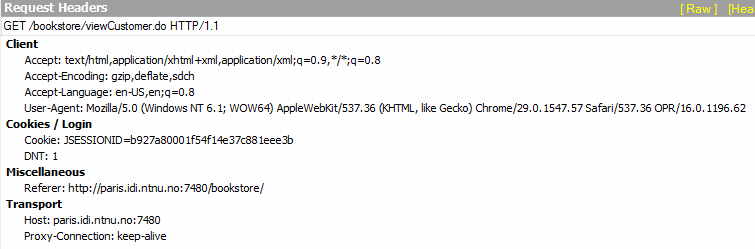
\includegraphics[scale=0.5]{pics/Reguest1.png}
\end{figure}

\begin{figure}[!ht]
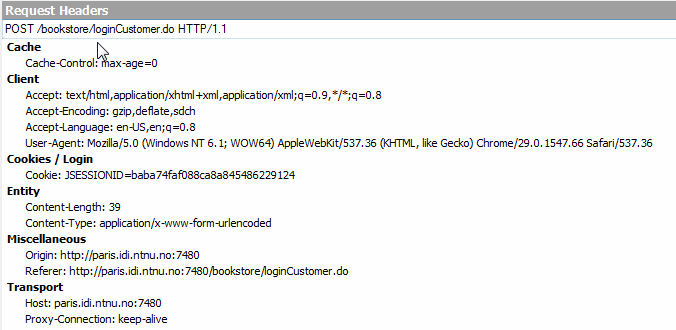
\includegraphics[scale=0.5]{pics/request2.png}
\end{figure}

\begin{figure}[!ht]
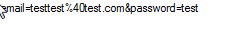
\includegraphics{pics/request10.png}
\end{figure}

\pagebreak

\subsection{Description of Tools}

{\bf Tools used during the black box testing:}
\begin{itemize}
	\item {\bf Fiddler:} HTTP debugging proxy server application, which captures and logs HTTP(S) traffic for the user to review. Can also be used for “fiddling” with HTTP-traffic as it is being sent.
	\item {\bf Webcruiser:} Web security software made by the security solution provider Janusec. Gives users the ability to discover possible vulnerabilities on web sites, by automatically scanning for vulnerabilities, such as Cross-site scripting and SQL injection.
	\item {\bf Brutus:} Online password cracker. Software that uses bruteforce attacks in order to discover several passwords that would be valid for a webpage. Brutus uses dictionary-based attacks for discovering these passwords.
	\item {\bf RainbowCrack:} Program for breaking hashes; generates and uses rainbow tables for a variety of character sets and hashing algorithms, including LM hash, MD5, SHA1, etc. It takes time to set up and create all rainbow chains, but it is supposed to break hash during a couple of minutes with high probability (99%).
	\item {\bf wget:} A tool that runs a recursive search through the website and downloads all files that are sent to the client side. We used this to draw up the pagemap, as well as looking for useful information.
	\item {\bf Web browser development tools:} Several web browsers (including Google Chrome, Mozilla FireFox, Internet Explorer) has a built-in development tool. These tools can be used for getting a good overview of a webpage’s CSS- and JavaScript- files, and inspecting the HTML-code more thoroughly. It also gives us the opportunity to manipulate the CSS- files.
	\item {\bf Edit This Cookie:} Plugin for Google Chrome browser to change the content of cookies.
	\item {\bf Sqlmap:} An open source penetration testing tool that automates the process of detecting and exploiting SQL injection flaws and taking over of database servers. We did try to use this, but we could not get it to work as we wanted.
	\item {\bf Metasploit:} A vulnerability and penetration testing software. Did not manage to use this tool because it was too complex to understand.
\end{itemize}

{\bf Tools Used During White Box Testing:}
\begin{itemize}
	\item {\bf VisualCodeGrepper} is an automated code security review tool for C++, C\#, VB, Java and PL/SQL, which examine code and finds insecure/bad code.
\end{itemize}

\newpage

\subsection{Pagemap}
In order to gather more information about the structure of the page, we created a pagemap. The green section shows which pages are accessible without being logged in, and the red section shows the pages which required being logged in to view. This can help us in planning the penetration tests, and understanding which pages are more vulnerable for attacks - the easiest is always to start with the pages that do not require authentication.

\begin{figure}[!ht]
\centering
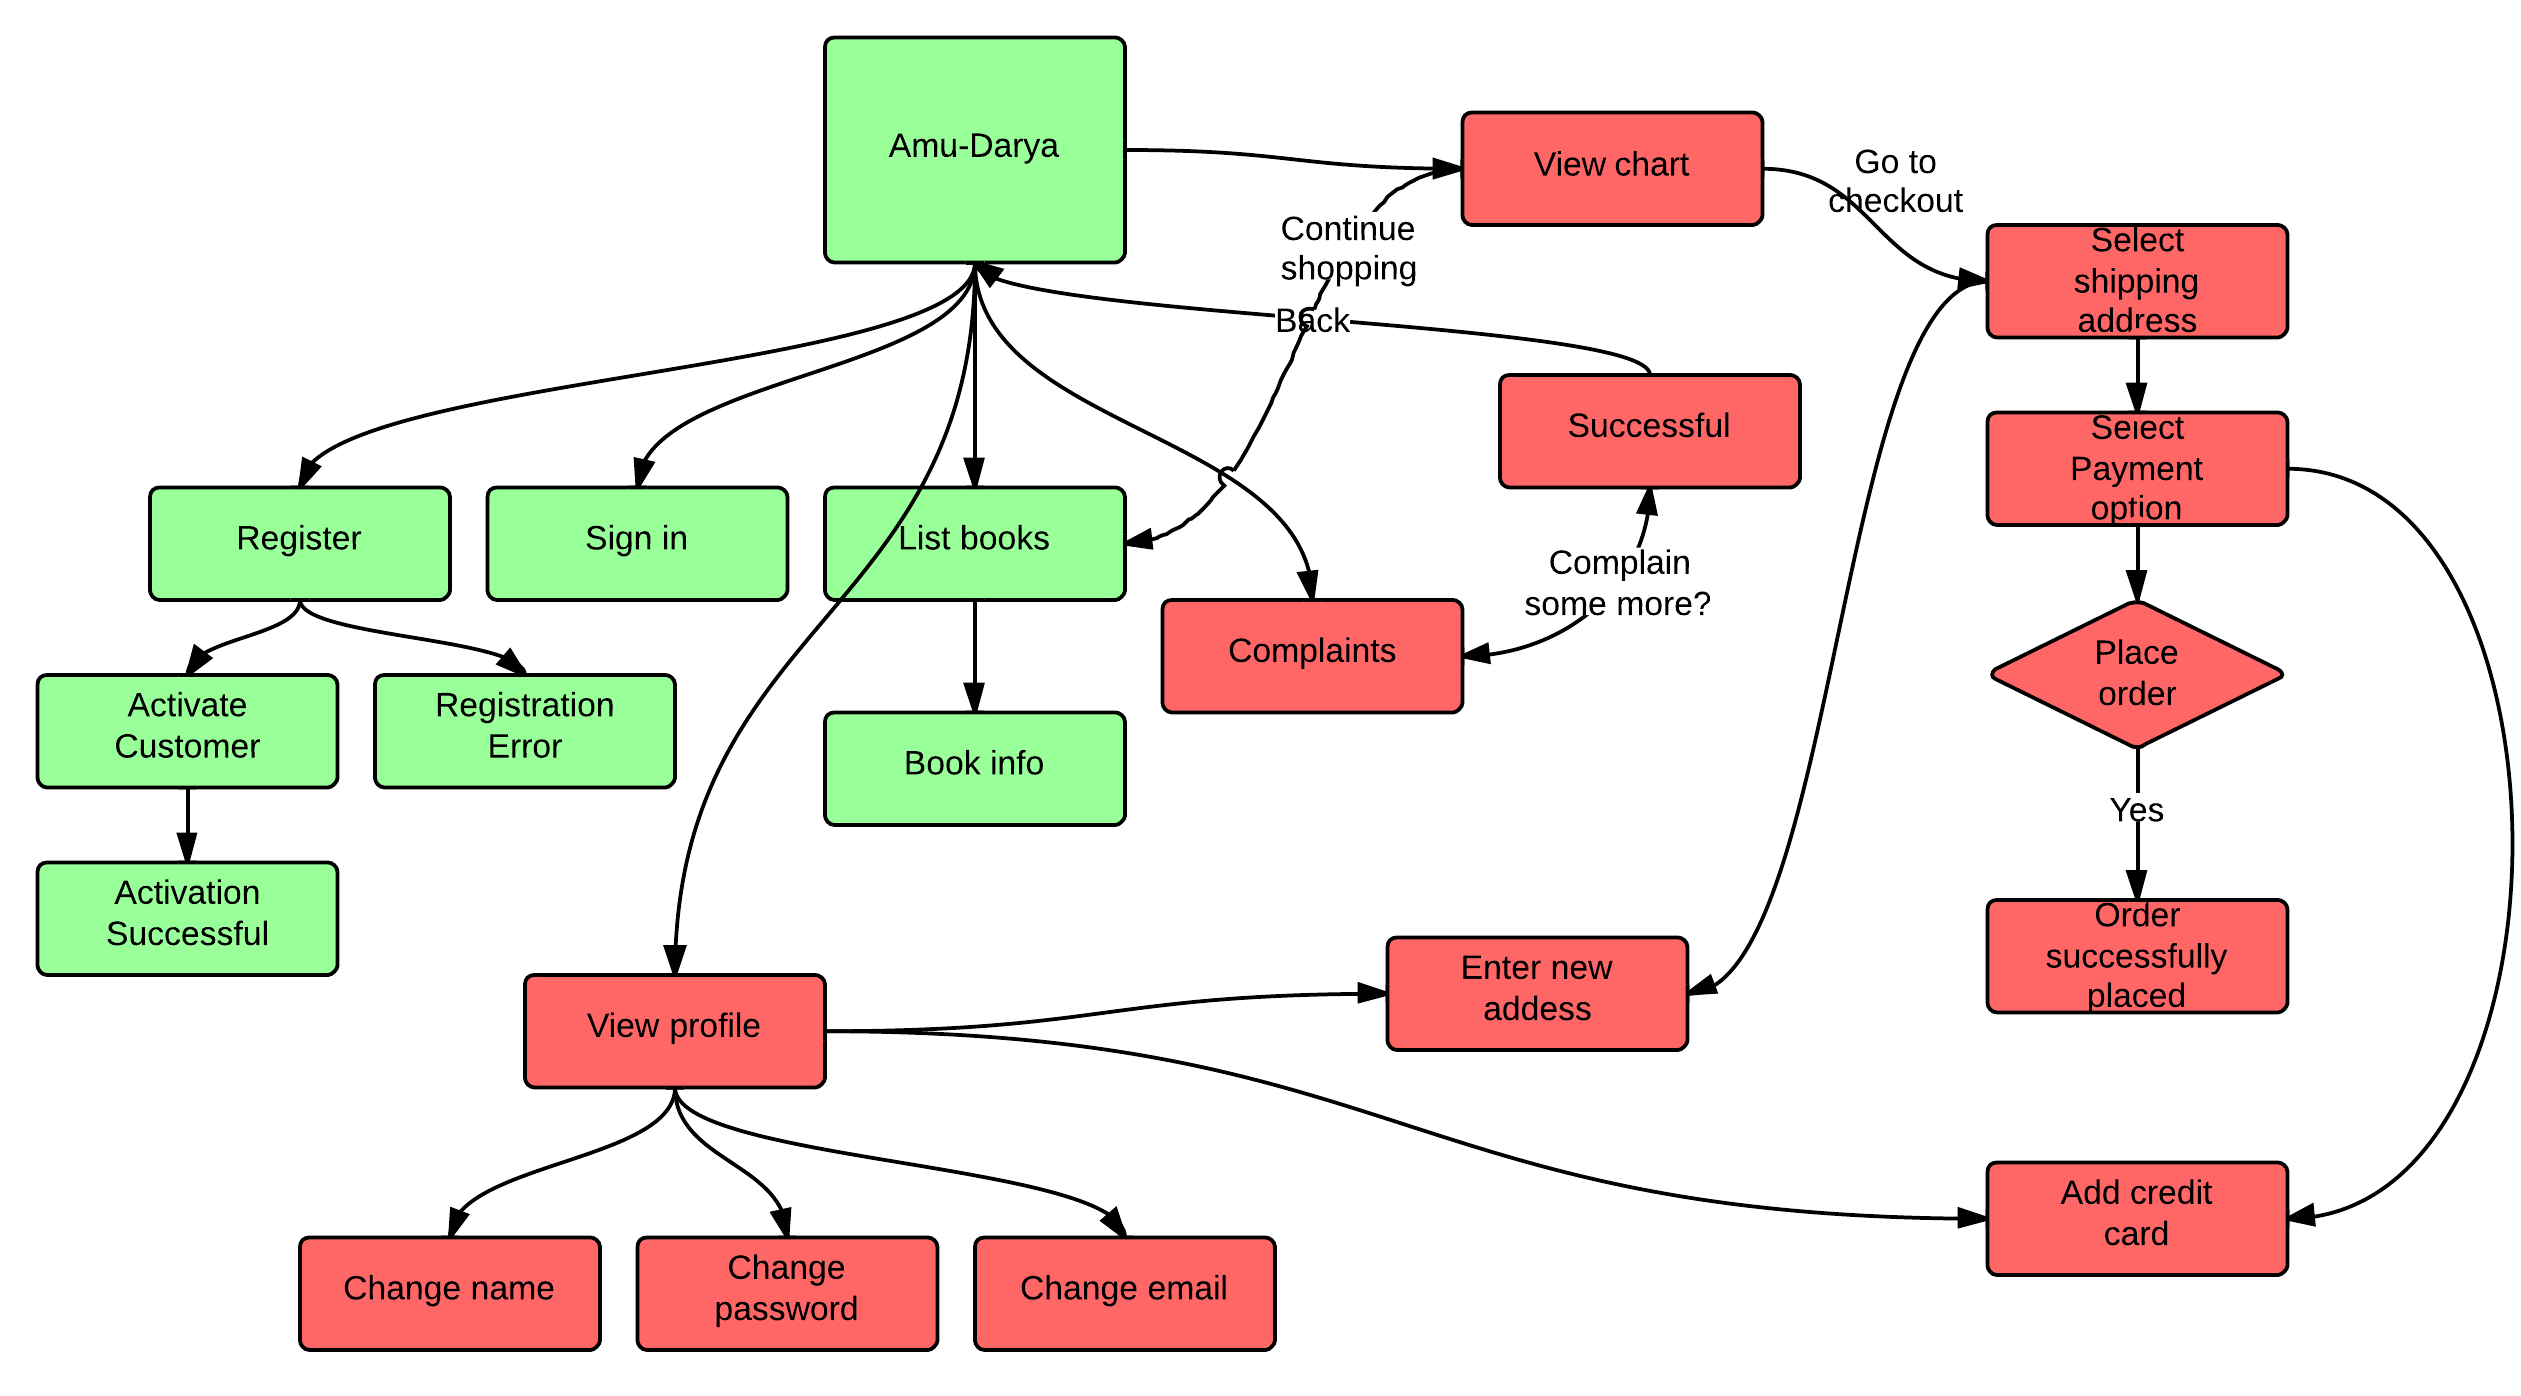
\includegraphics[scale=0.18, angle=90]{pics/Pagemap.png}
\end{figure}

{\bf Identifying Application Entry Points (OWASP-IG-003)}
To get a good understanding of the application and how the user communicates with it, we examined the web-page with Fiddler. We checked when GET- and POST-requests are used. We discovered some POST-parameters, GET-parameters and forms. There is a form on login screen, so we decided to do a brute force attack on it later. For POST-parameters we decided to use Fiddler to check what is sent and whether we could change something. For GET-parameters we made all changes directly in the URL to get a different result. We got quite often a server error code 500 when the input was of a wrong type, but this information was not very useful.
